\section{SIMULATION}
We use the rolling gait as the basic gait for the simulation. To verify the adaptive control of the robots in their motion, we simulate the robots' climbing on pipes with different diameters under the robot simulation platform VREP.

The simulation process can be divided into two categories: training and motion simulation. And we divide motion simulation into two parts: the adaptable motion along variable diameter pipes and the adaptable motion along straight pipes with different diameter .

\subsection{Training process}

In the data acquisition process, we make the robot climb along the 25cm and 35cm pipes for thousands of times respectively under different parameters. The interval of amplitude $A$, phase $\varepsilon$ and angular rate $\omega$ are $[40, \, 80]$, $[0, \, 5]$ and $[1.5, \, 3]$ respectively. What's more, the step of $A$ is 5, the step of $\varepsilon$ is 1 and the step of $\omega$ is 0.5. The state of the robot will change during the course of the movement. We make the robot climb with different combination of parameters and collect the data. Then we can eventually collect more than 20 thousand volumes of training data. In the preprocessing process, we cluster the training data. We set the number of clusters as 25. The number of data for most of classes is $1000 \pm 500 $ (\figref{fig:clustersize}).

\begin{figure}[t]
	\centering
	\includegraphics[width=0.6\linewidth]{fig/experiment/170912/cluster}
	\caption{The result of clustering}
	\figlabel{fig:clustersize}
\end{figure}

\subsection{the adaptable motion along variable diameter pipes}

The simulation in this part is 35cm to 25cm vertical pipe climbing simulation (\figref{fig:ccurve1}) and 25cm to 35cm vertical pipe climbing simulation (\figref{fig:ccurve2}). From the two simulation results we can find that the robot can adaptively learn to find better motion control parameters than current. Next, the two groups of simulation will be analyzed in detail.

\subsubsection{For 35cm to 25cm pipe climbing simulation}

The results are shown in \figref{fig:ccurve1}. In 0s to 15s, the robot changes itself from the stretch state to compressed state. Since the robot does not get the diameter of pipe, it spends a long time in adapting to the unknown pipe. So in this phase, its velocity is close to zero. In 15s to 40s, the robot climb along the pipe with 35cm diameter. In this phase, amplitude $A$, phase $\varepsilon$ and angular rate $\omega$ are all increasing and all of the them will be stable finally. About 50s, the robot reach the interface where the diameter changes. As the pipe changes obvious, the robot can not grasp the 25cm pipe immediately, which causes the velocity of the robot fluctuate around zero. The robot keeps learning and autonomously adjust its parameters to continue its climbing motion. From the \figref{fig:bsa} and \figref{fig:bsp}, it can be found that the amplitude and phase are increasing in this phase, which make the robot continue moving up.

Eventually all control parameters as well as velocity are stable. It shows that under this control strategy, the robot can adjust its parameters autonomously to adapt to the environment.

\begin{figure}[!t]
	\centering
	\subfigure[t= 0.0s]{
		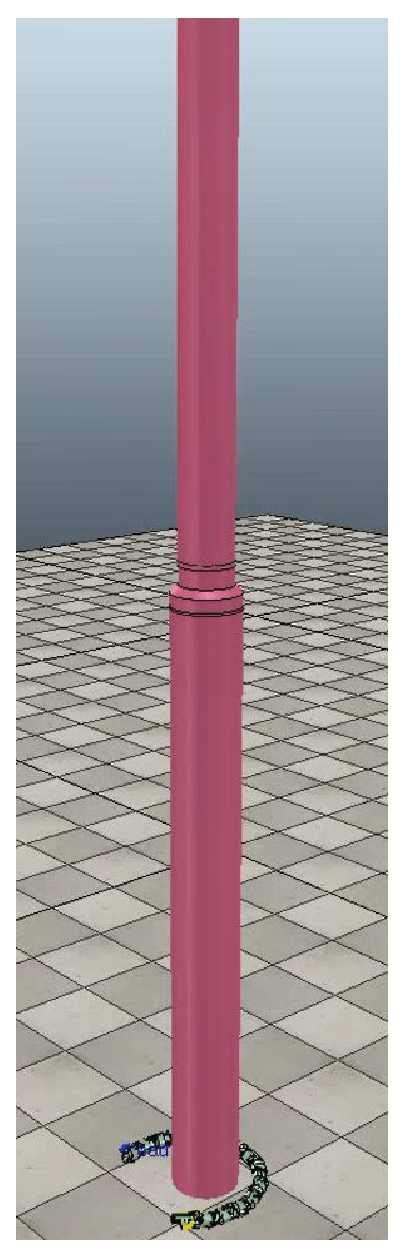
\includegraphics[height=2in,width=.12\textwidth]{fig/experiment/170912/bs0}
	}
	\subfigure[t=20.2s]{
		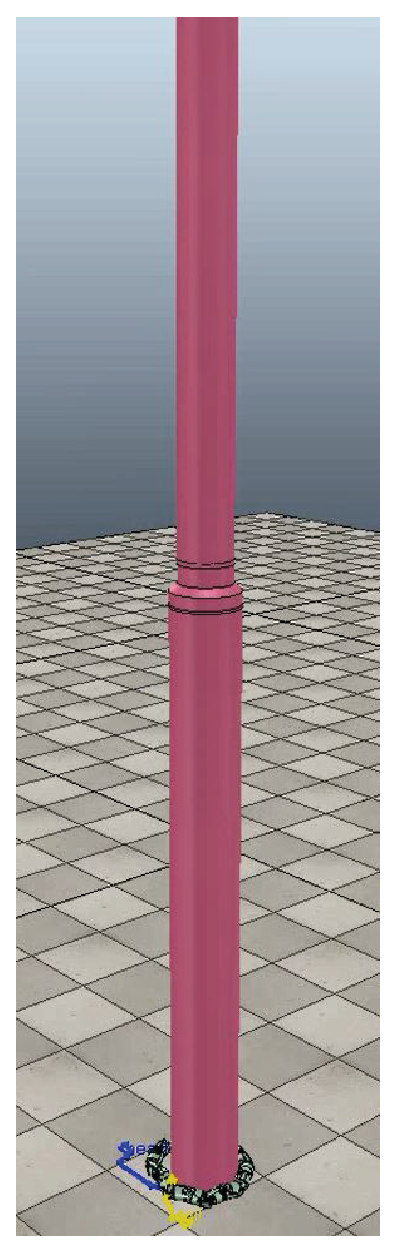
\includegraphics[height=2in,width=.12\textwidth]{fig/experiment/170912/bs1}
	}
	\subfigure[t=39.8s]{
		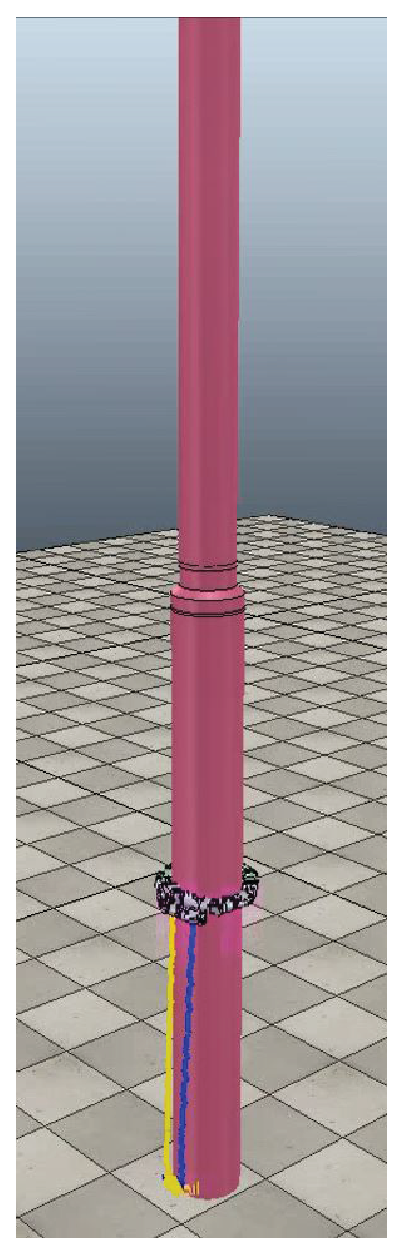
\includegraphics[height=2in,width=.12\textwidth]{fig/experiment/170912/bs2}
	}
	
	
	\subfigure[t=50.5s]{
		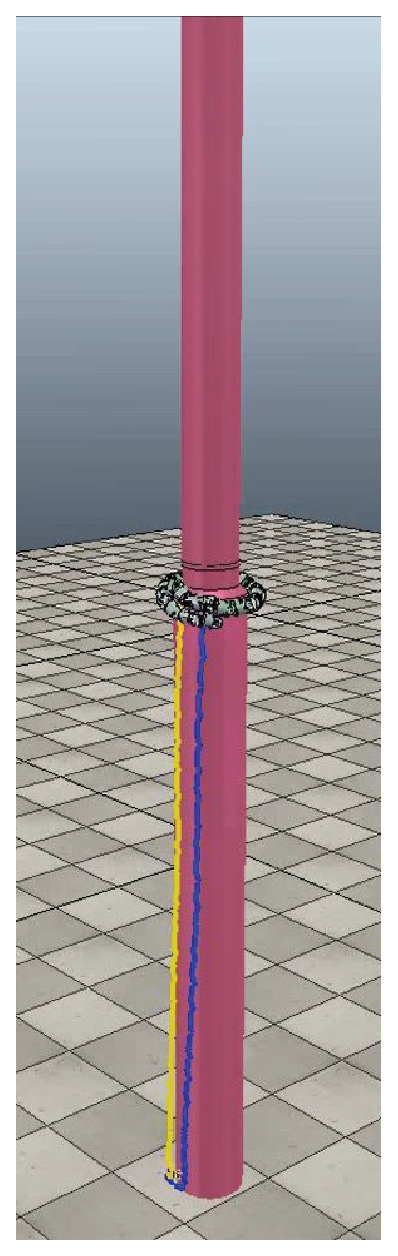
\includegraphics[height=2in,width=.12\textwidth]{fig/experiment/170912/bs3}
	}
	\subfigure[t=60.0s]{
		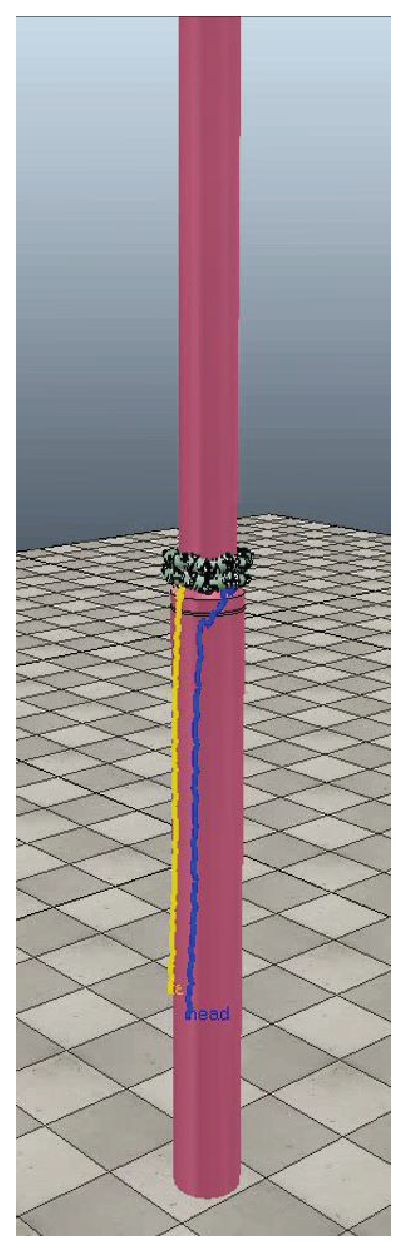
\includegraphics[height=2in,width=.12\textwidth]{fig/experiment/170912/bs4}
	}
	\subfigure[t=64.5s]{
		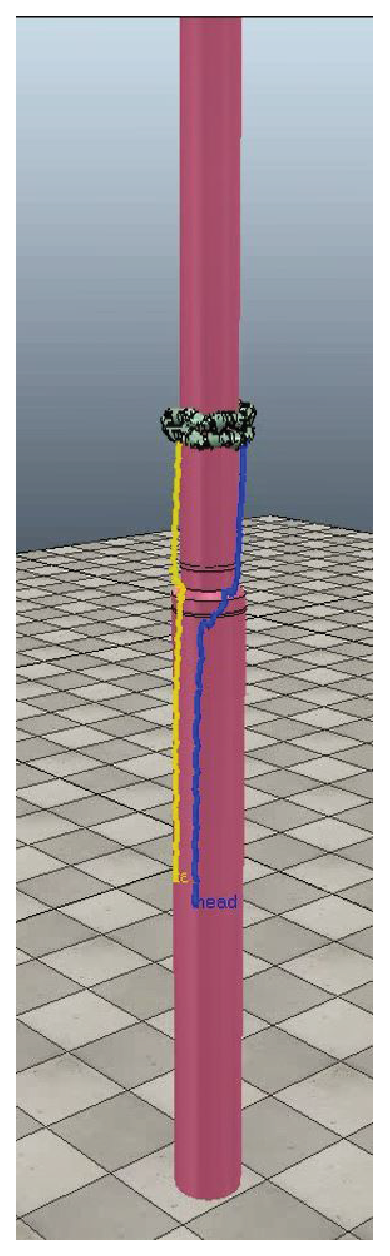
\includegraphics[height=2in,width=.12\textwidth]{fig/experiment/170912/bs5}
	}
	
	\subfigure[Amplifier versus Time]{
		\includegraphics[width=.2\textwidth]{fig/experiment/170912/bsamplifier}
		\figlabel{fig:bsa}
	}
	\subfigure[Phase versus Time]{
		\includegraphics[width=.2\textwidth]{fig/experiment/170912/bsphase}
		\figlabel{fig:bsp}
	}
	
	\subfigure[Angular rate versus Time]{
		\includegraphics[width=.2\textwidth]{fig/experiment/170912/bsangrate}
		\figlabel{fig:bsw}
	}
	\subfigure[velocity versus Time]{
		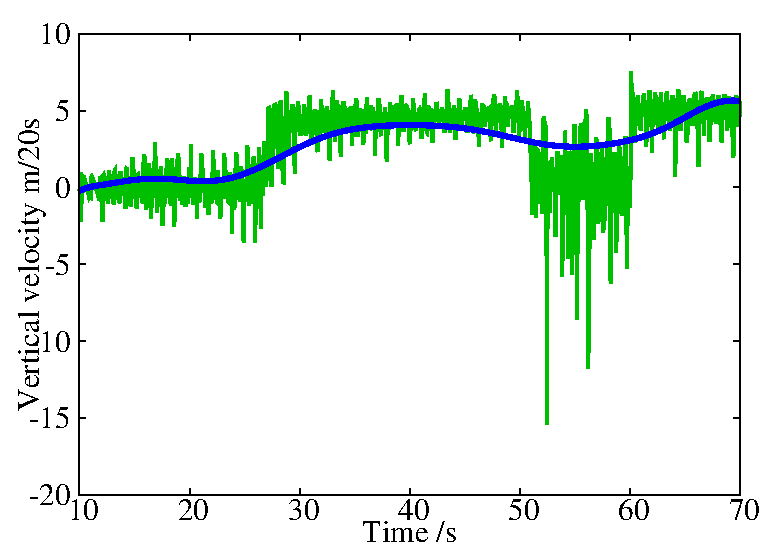
\includegraphics[width=.2\textwidth]{fig/experiment/170912/bsv}
		\figlabel{fig:bsv}
	}
	\caption{The movement process and the curves of parameters changing in the motion along the 35cm to 25cm pipe}
	\figlabel{fig:ccurve1}
\end{figure}

\begin{figure}[!t]
	\centering
	\subfigure[t= 0.0s]{
		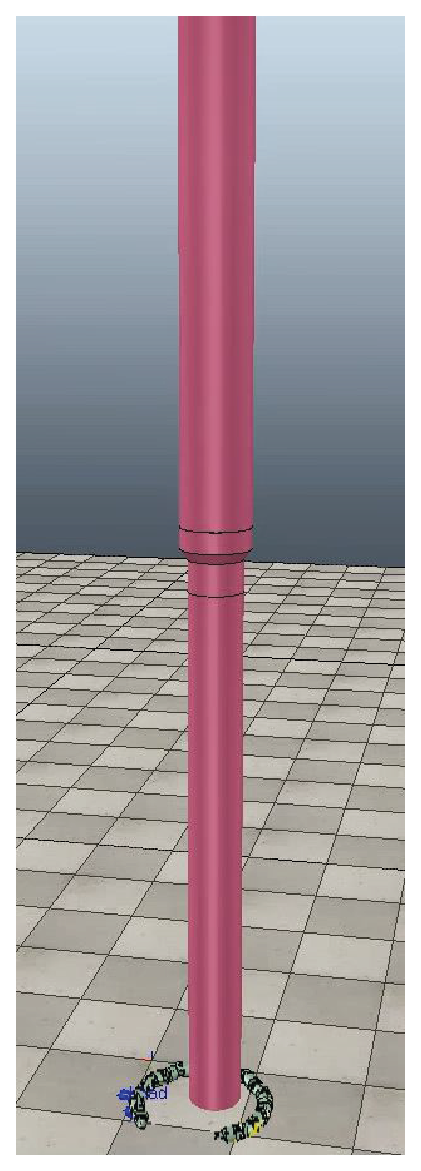
\includegraphics[height=2in,width=.12\textwidth]{fig/experiment/170912/sb0}
	}
	\subfigure[t=29.2s]{
		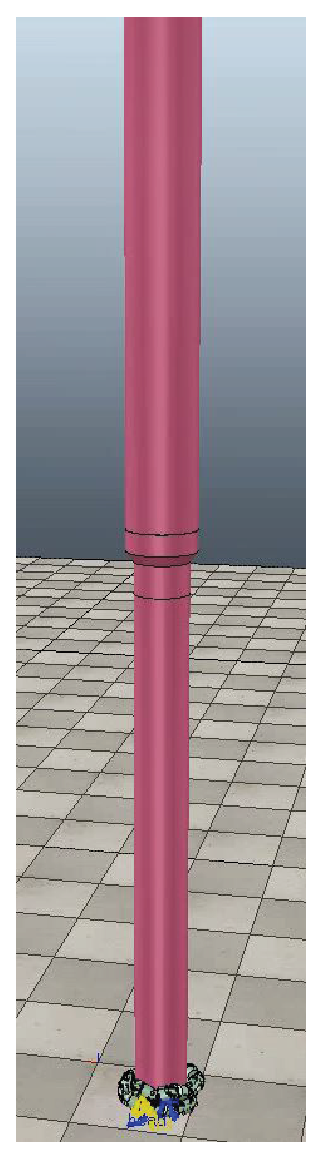
\includegraphics[height=2in,width=.12\textwidth]{fig/experiment/170912/sb1}
	}
	\subfigure[t=40.5s]{
		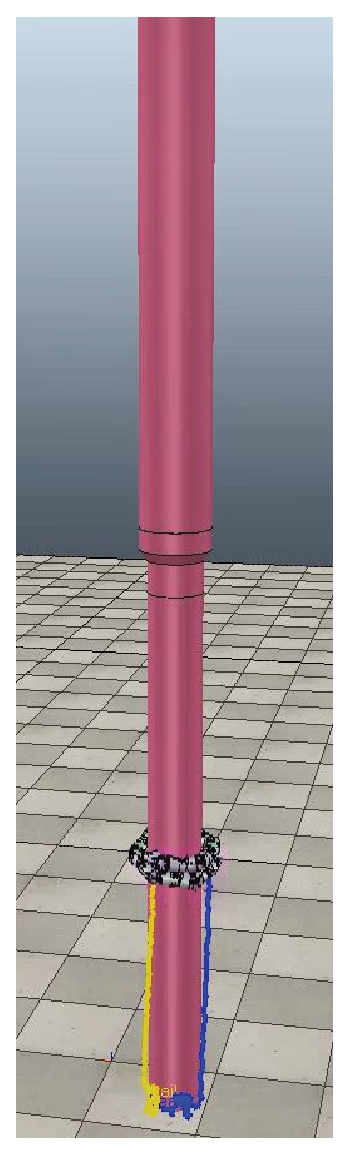
\includegraphics[height=2in,width=.12\textwidth]{fig/experiment/170912/sb2}
	}
	
	\subfigure[t=55.0s]{
		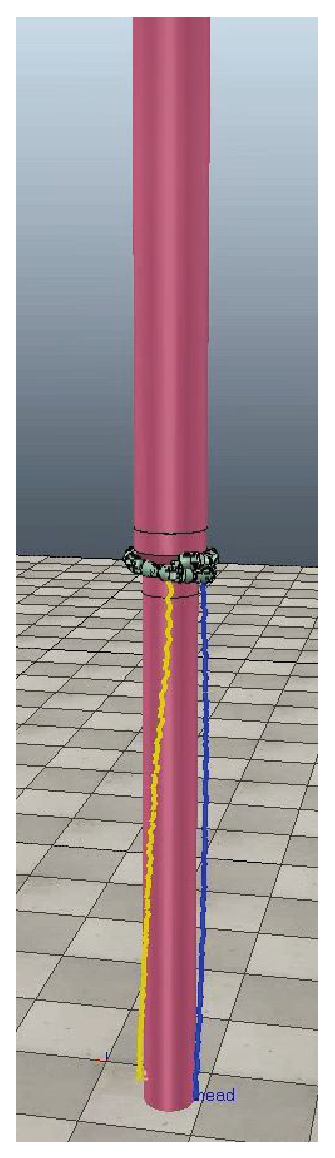
\includegraphics[height=2in,width=.12\textwidth]{fig/experiment/170912/sb3}
	}
	\subfigure[t=58.9s]{
		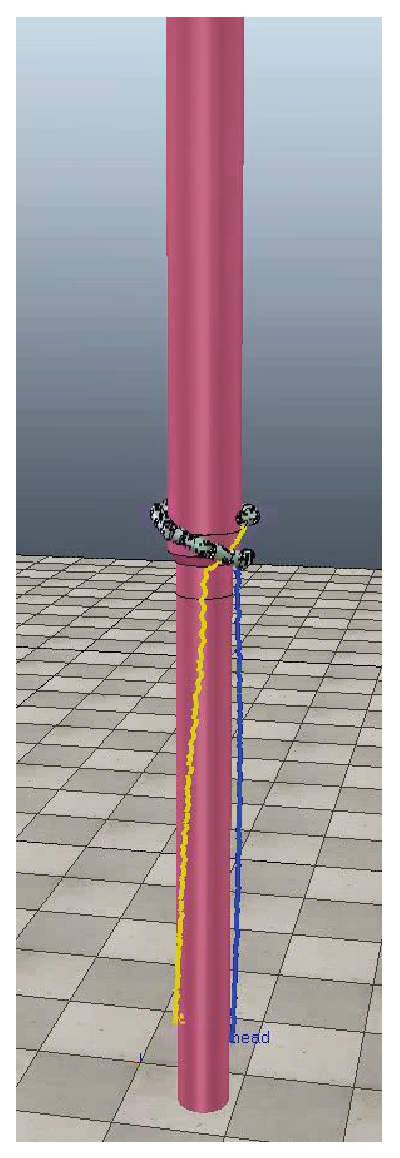
\includegraphics[height=2in,width=.12\textwidth]{fig/experiment/170912/sb4}
	}
	\subfigure[t=66.0s]{
		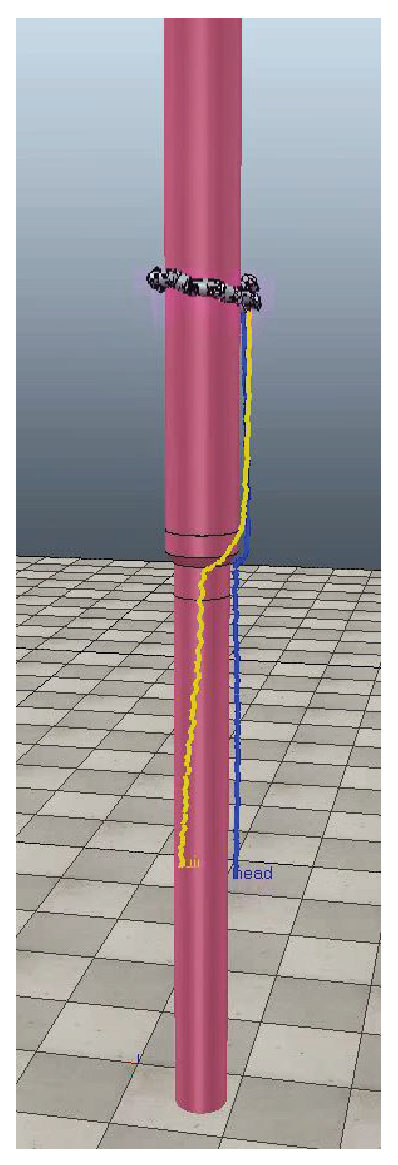
\includegraphics[height=2in,width=.12\textwidth]{fig/experiment/170912/sb5}
	}
	\subfigure[Amplifier versus Time]{
		\includegraphics[width=.2\textwidth]{fig/experiment/170912/sbamplifier1}
		\figlabel{fig:sba}
	}
	\subfigure[Phase versus Time]{
		\includegraphics[width=.2\textwidth]{fig/experiment/170912/sbphase}
		\figlabel{fig:sbp}
	}
	
	\subfigure[Angular rate versus Time]{
		\includegraphics[width=.2\textwidth]{fig/experiment/170912/sbangrate}
		\figlabel{fig:sbw}
	}
	\subfigure[velocity versus Time]{
		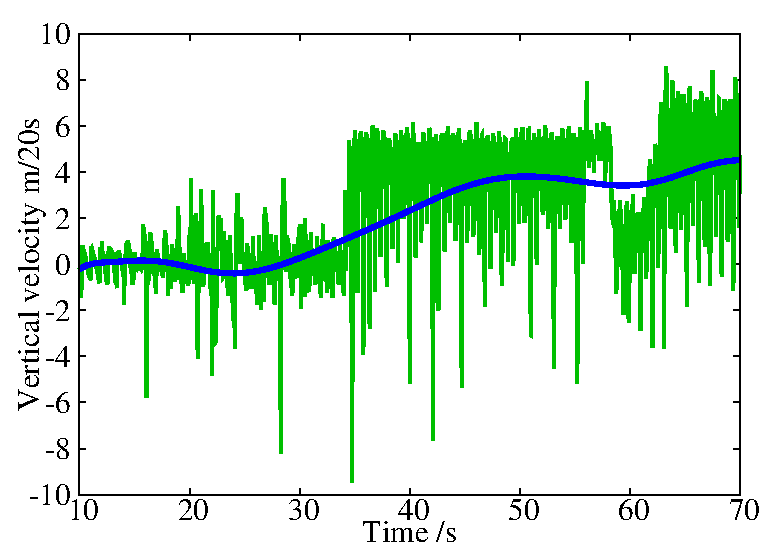
\includegraphics[width=.2\textwidth]{fig/experiment/170912/sbv}
		\figlabel{fig:sbv}
	}
	\caption{The movement process and the curves of parameters changing in the motion along the 25cm to 35cm pipe}
	\figlabel{fig:ccurve2}
\end{figure}

\subsubsection{For 25cm to 35cm pipe climbing simulation}
It is similar with the previous simulation, but the movement is different in the interface where the diameter changes. The results are shown in \figref{fig:ccurve2}. Firstly, the snake-like robot spend a lot of time to coil the 25cm pipeline. And then the robot adjust itself and finally its parameters reach stable. About 52s, the robot encounters the interface where the diameter changes. At this time the robot autonomously reduce amplitude slightly (\figref{fig:sba}) and then significantly increase  phase (\figref{fig:sbp}). In this way, the control strategy make the robot move itself from the 25cm part up to the 35cm part. When on the 35cm part, the robot will automatically increase the amplitude and decrease the phase shift until reaching the steady state.

Both simulations show that our method is effective to adapt the robot to climb along the variable diameter pipe.

\subsection{Contrast experiments on other straight pipes}

As the unknown environment in the real world is complex and volatile, there may be a movement environment different to the training environment. Our training environment is vertical pipes with 25cm or 35cm diameter. To ensure that this control strategy can be applied in many situation, we conduct several  independent simulations on 20cm, 25cm, 30cm, 35cm or 40cm straight pipe. The result of these simulations are shown in \figref{fig:scurve}. The simulations show that the robot can use our control strategy to catch the unknown pipe and adjust itself to a suitable climbing state. Next is the detailed analysis.

By observing the parameter curve we can find that the smaller diameter of the pipe is, the much more time the parameters need to spend in adjusting. All parameters finally reach a stable value and satisfy the requirements of movement. For the 40cm diameter pipe, the robot is not long enough to form a single ring to wrap the pipe (\figref{fig:D40}), in this case the influence made by phase $\varepsilon$ is very weak (\figref{fig:sphase}). For the 20cm diameter pipe, it is difficult for the robot to climb along the pipe only by increasing the amplitude $A$, because when the amplitude is too large, it will cause the snake-like robot curling up to a high degree, which is not conducive to climb. Therefore, to make the robot climb small diameter pipe, we need to constantly adjust the phase $\varepsilon$ to meet the amplitude $A$'s corresponding requirements. By observing the variation curve of the control parameters of the small diameter pipe, we can found that the phase $\varepsilon$ and the amplitude $A$ of the robot are coordinated in the process of self-regulation ( \figref{fig:samplifier})(\figref{fig:sphase}).

\begin{figure}[!t]
	\centering
	\subfigure[d=20cm]{
		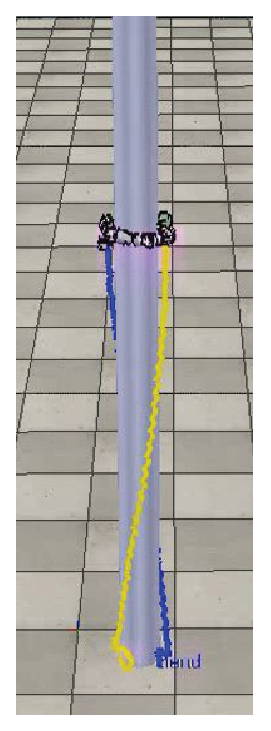
\includegraphics[height=2in,width=.12\textwidth]{fig/experiment/170912/D20}
		\figlabel{fig:D20}
	}
	\subfigure[d=25cm]{
		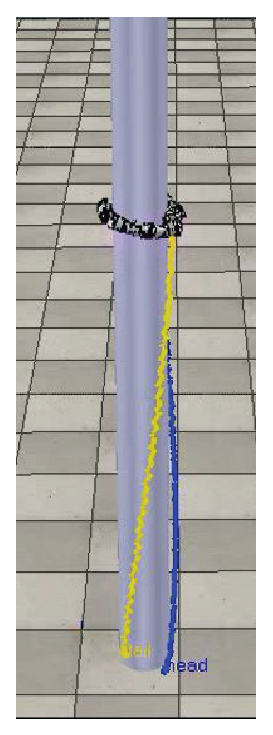
\includegraphics[height=2in,width=.12\textwidth]{fig/experiment/170912/D25}
		\figlabel{fig:D25}	
	}
	
	\subfigure[d=30cm]{
		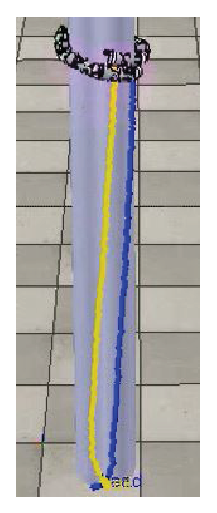
\includegraphics[height=2in,width=.12\textwidth]{fig/experiment/170912/D30}
		\figlabel{fig:D30}
	}
	\subfigure[d=35cm]{
		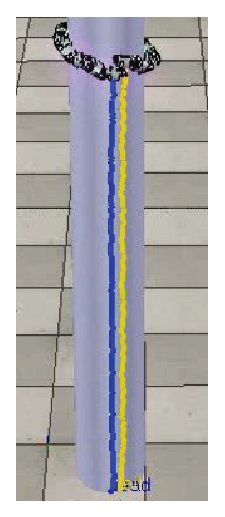
\includegraphics[height=2in,width=.12\textwidth]{fig/experiment/170912/D35}
		\figlabel{fig:D35}
	}
	\subfigure[d=40cm]{
		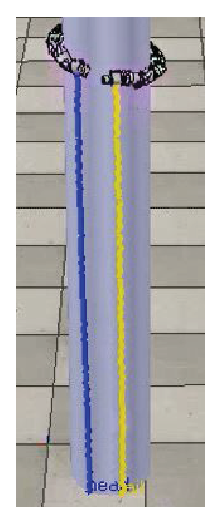
\includegraphics[height=2in,width=.12\textwidth]{fig/experiment/170912/D40}
		\figlabel{fig:D40}
	}
	
	\subfigure[Amplifier versus Time]{
		\includegraphics[width=.2\textwidth]{fig/experiment/170912/samplifier}
		\figlabel{fig:samplifier}
	}
	\subfigure[Phase versus Time]{
		\includegraphics[width=.2\textwidth]{fig/experiment/170912/sphase}
		\figlabel{fig:sphase}
	}
	\subfigure[Angular rate versus Time]{
		\includegraphics[width=.2\textwidth]{fig/experiment/170912/sarate}
		\figlabel{fig:sarate}
	}
	\subfigure[velocity versus Time]{
		\includegraphics[width=.2\textwidth]{fig/experiment/170912/svel}
		\figlabel{fig:svelocity}
	}
	\caption{The comparison curve about parameters changing versus time in different diameter pipe climbing}
	\figlabel{fig:scurve}
\end{figure}

It is worth noting that, for all test environments, the movement velocity of the robot ultimately fluctuate within a constant range  (\figref{fig:svelocity}). The diameter of the pipe only affects the velocity convergence rate. And also the control parameters of the robot will eventually become stable (\figref{fig:scurve}). This shows that the influence of the external environment to this control strategy is very weak. What's more, the robot will find the optimal parameter during its motion.

The above simulations show that our control strategy can be applied to a lot of environment and is effective, too.

In conclusion, the simulations demonstrate that the adaptive control in robot's motion can be realized through our proposed framework in \figref{fig:stepMap}.
